\chapter{El cerebro al mando}\label{ch:g5:brain-in-command}

Una pelota vuela hacia ti; la coges. Medio segundo, sin pensar nada
--- y sin embargo, en ese medio segundo tus \omterm{def:g1:the-five-senses:sense}{ojos} informaron de un
objeto volando, algo calculó su trayectoria y decenas de \omterm{def:g3:bones-and-muscles:muscle}{músculos}
recibieron la orden de hacer exactamente la parada correcta. Ese algo
es el \omterm{def:g5:brain-in-command:system}{cerebro}, y este capítulo sigue sus órdenes por el cableado del
cuerpo.

\section{La red de mando}

\begin{definition}[El sistema nervioso]\label{def:g5:brain-in-command:system}
El \emph{sistema nervioso}\index{sistema nervioso} es la red de mando
del cuerpo:
\begin{itemize}
  \item el \emph{cerebro}\index{cerebro}, al abrigo del \omterm{def:g3:bones-and-muscles:skeleton}{cráneo}
        (\cref{def:g3:bones-and-muscles:skeleton}), es el centro:
        recibe todos los informes y da todas las órdenes;
  \item la \emph{médula espinal}\index{médula espinal}, un cable
        grueso de tejido nervioso, baja desde el cerebro por dentro de
        la columna protectora de la espalda;
  \item los \emph{nervios}\index{nervio}, hilos blancos que se
        ramifican desde el cerebro y la médula hasta todos los
        órganos, llevan los mensajes --- a más de \qty{100}{m/s} los
        más rápidos.
\end{itemize}
\end{definition}

\begin{proposition}[Informar, decidir, ordenar]\label{prop:g5:brain-in-command:loop}
Todas las acciones recorren el mismo bucle (la
\cref{prop:g1:the-five-senses:brain} fue su primer esbozo):
\begin{enumerate}
  \item los \emph{\omterm{def:g1:the-five-senses:sense}{órganos de los sentidos}} informan: los \omterm{def:g5:brain-in-command:system}{nervios}
        llevan sus mensajes \emph{hasta} el \omterm{def:g5:brain-in-command:system}{cerebro};
  \item el \emph{\omterm{def:g5:brain-in-command:system}{cerebro}} junta los informes, decide y compone unas
        órdenes;
  \item los \omterm{def:g5:brain-in-command:system}{nervios} llevan las órdenes \emph{desde} el \omterm{def:g5:brain-in-command:system}{cerebro} hasta
        los \emph{\omterm{def:g3:bones-and-muscles:muscle}{músculos}} (\cref{def:g3:bones-and-muscles:muscle}),
        que se contraen a la orden.
\end{enumerate}
Los \omterm{def:g1:the-five-senses:sense}{órganos de los sentidos} informan y los \omterm{def:g3:bones-and-muscles:muscle}{músculos} obedecen ---
ninguno de los dos decide nunca.
\end{proposition}
\admitted

\begin{omfigure}
\begin{tikzpicture}
  % eye
  \draw[thick] (-0.7,1.7) ellipse (0.5 and 0.28);
  \fill[omDef] (-0.58,1.7) circle (0.13);
  \node[font=\small, align=center] (eye) at (-0.7,0.85)
    {el ojo ve\\ la pelota};
  % brain
  \draw[thick, omDef, fill=omDef!8, rounded corners=8pt]
    (3.2,1.15) rectangle (6.4,2.45);
  \node[font=\small\bfseries, omDef] at (4.8,2.05) {el cerebro};
  \node[font=\footnotesize] at (4.8,1.55) {decide la parada};
  % muscle
  \draw[thick, omThm, fill=omThm!15]
    (9.6,1.5) .. controls (10.0,1.85) and (10.6,1.85) .. (11.0,1.55)
    .. controls (10.6,1.35) and (10.0,1.35) .. (9.6,1.5);
  \node[font=\small, align=center] at (10.3,0.85)
    {los músculos del brazo\\ se contraen};
  % arrows
  \draw[->, very thick, omMeth] (-0.1,1.7) -- (3.1,1.8)
    node[pos=0.42, above=2pt, font=\footnotesize, omMeth]
    {informe, por un nervio};
  \draw[->, very thick, omProp] (6.5,1.8) -- (9.5,1.6)
    node[pos=0.5, above=2pt, font=\footnotesize, omProp]
    {orden, por un nervio};
\end{tikzpicture}

{\small El bucle de toda acción: informe al \omterm{def:g5:brain-in-command:system}{cerebro}, decisión, orden a
los \omterm{def:g3:bones-and-muscles:muscle}{músculos}.}
\end{omfigure}

\begin{example}[La parada, repetida a cámara lenta]\label{ex:g5:brain-in-command:catch}
Repite el medio segundo: los \omterm{def:g1:the-five-senses:sense}{ojos} siguen la pelota e informan sin
parar; el \omterm{def:g5:brain-in-command:system}{cerebro}, comparando informe tras informe, calcula dónde
estará la pelota; salen órdenes en cadena hacia las \omterm{def:g1:my-body:parts}{piernas} (un paso a
la izquierda), el tronco (inclinarse), el \omterm{def:g1:my-body:parts}{brazo} y los dedos (abrir ---
ahora cerrar). Ningún órgano ``cogió la pelota'' él solo: los \omterm{def:g1:the-five-senses:sense}{ojos}, el
\omterm{def:g5:brain-in-command:system}{cerebro} y los \omterm{def:g3:bones-and-muscles:muscle}{músculos} hicieron cada uno su línea de la
\cref{prop:g5:brain-in-command:loop}.
\end{example}

\begin{remark}[Más que movimiento]\label{rem:g5:brain-in-command:more}
El mismo \omterm{def:g5:brain-in-command:system}{cerebro} que coge pelotas guarda además tus recuerdos,
mantiene tu atención en esta página, sueña por la noche --- y lleva
servicios en los que no piensas nunca: mantiene la \omterm{def:g4:breathing:movements}{respiración} en
marcha día y noche (\cref{def:g4:breathing:movements}) y ajusta el
ritmo del \omterm{def:g4:heart-and-blood:heart}{corazón} a lo que el cuerpo necesita
(\cref{ex:g4:heart-and-blood:effort}). Unas órdenes las das tú; otras
las da el \omterm{def:g5:brain-in-command:system}{cerebro} por ti.
\end{remark}

\section{Medir el bucle: el tiempo de reacción}

\begin{definition}[Tiempo de reacción]\label{def:g5:brain-in-command:reaction}
El bucle es rápido, pero no instantáneo: el informe, la decisión y la
orden se llevan cada uno su parte. El retraso entre una señal y la
respuesta del cuerpo es el \emph{tiempo de reacción}\index{tiempo de
reacción} --- para una tarea sencilla (coger, pulsar, agarrar), como
un quinto de segundo en una persona entrenada, y un poco más en los
niños.
\end{definition}

\begin{method}[La prueba de la regla]\label{met:g5:brain-in-command:ruler}
El \omterm{def:g5:brain-in-command:reaction}{tiempo de reacción} sin más instrumento que una regla:
\begin{enumerate}
  \item alguien sujeta una regla colgando en vertical, con el cero
        abajo, entre tu pulgar y tu dedo abiertos;
  \item sin avisar, la suelta; tú coges la regla lo más deprisa que
        puedas;
  \item lee por dónde la has cogido: cuantos menos centímetros se
        hayan escapado, más rápido es tu bucle;
  \item repítelo varias veces y quédate con tu valor habitual --- los
        intentos sueltos dan saltos.
\end{enumerate}
La regla que cae convierte el tiempo en centímetros: unos
$\qty{15}{cm}$ corresponden a un sexto de segundo.
\end{method}

\begin{omfigure}
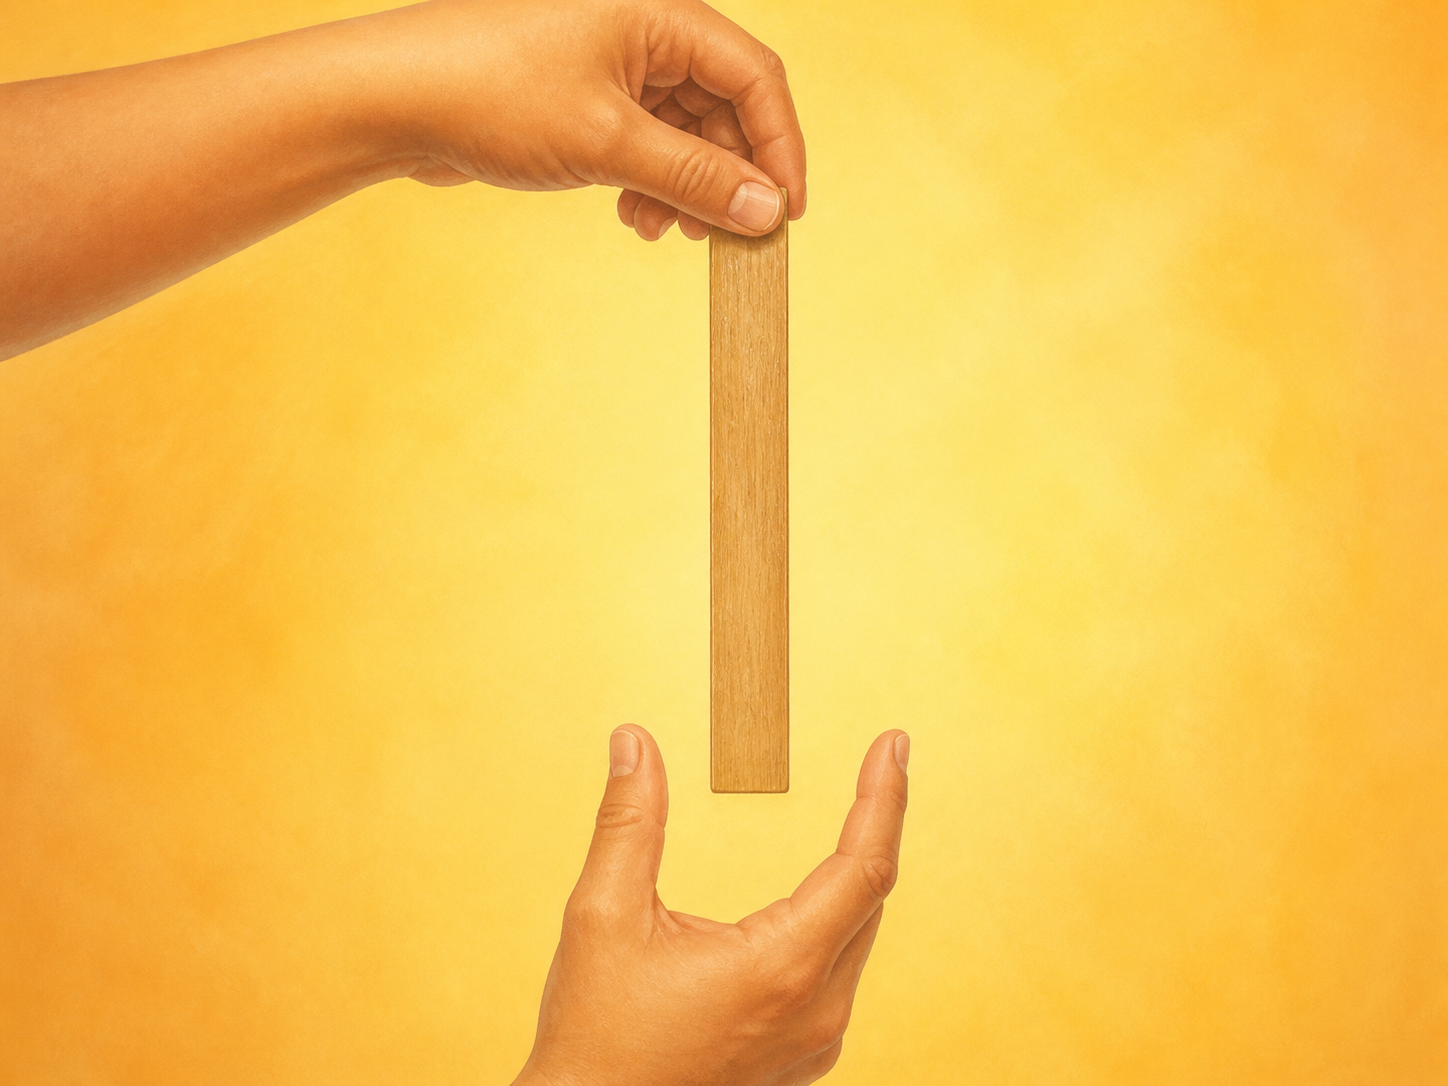
\includegraphics[width=0.5\linewidth]{images/book1/ai/g5-brain-ruler.png}

{\small La prueba de la regla, un instante antes de la soltada: cuando
la mano de arriba suelta, el bucle de la de abajo --- ver, decidir,
cerrar --- arranca su quinto de segundo.}
\end{omfigure}

\begin{example}[Por qué el asiento del copiloto es el primero que grita]\label{ex:g5:brain-in-command:driver}
Un quinto de segundo no parece nada --- hasta que la velocidad lo
multiplica. Un coche a velocidad de autovía recorre unos \qty{7}{m}
durante una reacción de un quinto de segundo: el conductor todavía no
ha tocado el freno y el coche ya ha cruzado un aula. El \omterm{def:g5:brain-in-command:reaction}{tiempo de
reacción} es la razón de que existan las distancias entre coches, y de
que la atención de un conductor sea un órgano de seguridad.
\end{example}

\begin{remark}[Entrenar el bucle]\label{rem:g5:brain-in-command:training}
La práctica acorta y afina el bucle --- no la velocidad de los
\omterm{def:g5:brain-in-command:system}{nervios}, sino el enrutado del \omterm{def:g5:brain-in-command:system}{cerebro}. La malabarista principiante se
lo cae todo; un mes después, el mismo \omterm{def:g5:brain-in-command:system}{cerebro} guía las mismas manos
por tres pelotas sin esfuerzo aparente. Aprender una destreza es el
\omterm{def:g5:brain-in-command:system}{cerebro} trazando mejores caminos --- otra cosa más que crece con el
ejercicio, como los \omterm{def:g3:bones-and-muscles:muscle}{músculos} del
\cref{met:g3:bones-and-muscles:care}.
\end{remark}

\section{Proteger al que manda}

\begin{proposition}[Sueño, comida, seguridad]\label{prop:g5:brain-in-command:protect}
El \omterm{def:g5:brain-in-command:system}{cerebro} es el órgano más protegido del cuerpo --- casco de \omterm{def:g3:bones-and-muscles:skeleton}{cráneo},
columna de la espalda --- y el más exigente: aunque es una parte
pequeña del peso del cuerpo, consume una parte grande de su \omterm{prop:g3:balanced-diet:jobs}{energía} y
de su oxígeno (\cref{prop:g4:heart-and-blood:carries}), y hace sus
archivos y sus reparaciones durante el \emph{\omterm{prop:g1:healthy-habits:needs}{sueño}}
(\cref{prop:g1:healthy-habits:needs}). Un \omterm{def:g5:brain-in-command:system}{cerebro} cansado manda mal:
reacciones más lentas, atención dispersa, decisiones de mal humor.
\end{proposition}
\admitted

\begin{example}[Los cascos son para el bucle]\label{ex:g5:brain-in-command:helmet}
Los \omterm{def:g3:bones-and-muscles:skeleton}{huesos} se sueldan (\cref{rem:g3:bones-and-muscles:alive}); el
tejido del \omterm{def:g5:brain-in-command:system}{cerebro}, una vez dañado de gravedad, casi nunca. Ese es el
cálculo que hay detrás de los cascos de bicicleta: \omterm{def:g3:bones-and-muscles:skeleton}{cráneo} más espuma
allí donde la protección del propio cuerpo podría no bastar. Un seguro
barato para el órgano que dirige todo lo demás.
\end{example}

\section{Ejercicios}

\begin{exercise}[$\star$]\label{exo:g5:brain-in-command:1}
Nombra las tres partes del \omterm{def:g5:brain-in-command:system}{sistema nervioso} y el papel de cada una.
\end{exercise}

\begin{exercise}[$\star$]\label{exo:g5:brain-in-command:2}
Enuncia el bucle de toda acción en tres pasos. ¿Qué partes informan,
cuál decide y cuáles obedecen?
\end{exercise}

\begin{exercise}[$\star$]\label{exo:g5:brain-in-command:3}
¿Dónde están protegidos el \omterm{def:g5:brain-in-command:system}{cerebro} y la \omterm{def:g5:brain-in-command:system}{médula espinal}, y por qué
\omterm{def:g3:bones-and-muscles:skeleton}{huesos}?
\end{exercise}

\begin{exercise}[$\star$]\label{exo:g5:brain-in-command:4}
¿Qué es el \omterm{def:g5:brain-in-command:reaction}{tiempo de reacción}? Da su valor aproximado para una tarea
sencilla.
\end{exercise}

\begin{exercise}[$\star$]\label{exo:g5:brain-in-command:5}
Repite a cámara lenta, como en el \cref{ex:g5:brain-in-command:catch}:
pisas algo puntiagudo y tu pie se aparta de un tirón. ¿Quién informó,
quién decidió y quién obedeció?
\end{exercise}

\begin{exercise}[$\star$]\label{exo:g5:brain-in-command:6}
Da dos servicios que lleva el \omterm{def:g5:brain-in-command:system}{cerebro} sin que tú pienses en ellos,
sacados de la \cref{rem:g5:brain-in-command:more}.
\end{exercise}

\begin{exercise}[$\star$]\label{exo:g5:brain-in-command:7}
¿Por qué manda mal un \omterm{def:g5:brain-in-command:system}{cerebro} cansado? Nombra dos de sus necesidades a
partir de la \cref{prop:g5:brain-in-command:protect}.
\end{exercise}

\begin{exercise}[$\star$]\label{exo:g5:brain-in-command:8}
Pruébalo: haz la prueba de la regla del
\cref{met:g5:brain-in-command:ruler}, cinco intentos. Da tu distancia
de agarre habitual --- y di si la práctica la mejoró.
\end{exercise}

\begin{exercise}[$\star\star$]\label{exo:g5:brain-in-command:9}
¿Por qué no existe la parada instantánea, por muy hábil que sea quien
coge? Responde con los tres pasos del bucle.
\end{exercise}

\begin{exercise}[$\star\star$]\label{exo:g5:brain-in-command:10}
Con el \cref{ex:g5:brain-in-command:driver}: ¿por qué exigen las
normas de tráfico \emph{distancia} entre coches y no solo buenos
frenos? ¿Qué cambia la atención dentro del bucle?
\end{exercise}

\begin{exercise}[$\star\star\star$]\label{exo:g5:brain-in-command:11}
La malabarista de la \cref{rem:g5:brain-in-command:training} mejoró sin
que sus \omterm{def:g5:brain-in-command:system}{nervios} condujeran más deprisa. ¿Qué parte del bucle mejoró
entonces? Compáralo con entrenar un \omterm{def:g3:bones-and-muscles:muscle}{músculo}: ¿qué crece en cada caso?
\end{exercise}
